\documentclass[style=upen, size=14pt]{powerdot}
\usepackage{natbib}
\usepackage{bibentry}
\usepackage{mathtools}
\definecolor{arany}{RGB}{255,242,0}
\hypersetup{backref=page}
\hypersetup{
    colorlinks=true,
    linkcolor=cyan,
    citecolor=cyan,
    filecolor=magenta,      
    urlcolor=cyan}
% \pdsetup{trans=Split}
\usepackage{graphicx}
\usepackage{amsmath}
\DeclareMathOperator*{\argmax}{argmax}
\DeclareMathOperator*{\argmin}{argmin}
\DeclareMathOperator*{\softmax}{softmax}
\DeclareMathOperator{\sign}{sign}
\usepackage{amssymb}
\usepackage{stmaryrd}
\usepackage[latin2]{inputenc}
%\usepackage[magyar]{babel}
%\usepackage{euler}
\usepackage{tikz}
\usetikzlibrary{matrix}
\usepackage{tikz-qtree}
\usepackage{tikz-dependency}
\usepackage{linguex}
\usepackage{amsthm}
\usepackage{amsmath}
%\tikzset{every tree node/.style={align=center,anchor=north}}
%\usepackage{tabularx}
%\usepackage{threeparttable}
%\usepackage{color}
%\selectlanguage{english}
%\frenchspacing
\usepackage{algpseudocode}
\usepackage{algorithm}
\newcommand\varlist{,\makebox[1em][c]{.\hfil.\hfil.},}
\newcommand{\nd}{\noindent}
\newcommand{\Val}{\mathop{\mathit{Val}}}
\newcommand{\gold}{\color{arany}}
%\usepackage{tikz}
%\usepackage{tikz-qtree}
%\newcommand{\qed}{\hfill\mbox{\raggedright \rule{.1in}{.1in}}}
\def\es{\mathbin\land}
\theoremstyle{definition}
\newtheorem*{definition}{Definition}
\newtheorem{axioma}{Axiom}
\newtheorem{tetel}{Theorem}
\newtheorem{prop}{Proposition}
\newtheorem{lemma}{Lemma}
\begin{document}

\title{Natural Language Processing\\~~\\Lecture 6\\Dependency parsing}
% \author{}

\date{2021}
\maketitle

\section{The dependency parsing task}

\begin{slide}[toc=Syntactic parsing]{Syntactic parsing (refresher)}
  Syntactic theories aim to characterize

  \begin{quote}
  ``the set of rules or principles that
  govern how words are put together to form phrases, well formed sequences of
  words.'' \citep[1]{koopman2013introduction}
\end{quote}

  The most important ``well formed sequences'' in this context are
  \emph{sentences}: the central goal of syntactic theories for a given language
  is to find structural rules or principles that characterize/delineate well
  formed sentences of the language in question.
\end{slide}

\begin{slide}[toc=]{Syntactic parsing cont.}
  A sentence is well formed if it has a \emph{structural description} or
  \emph{syntactic parse} which satisfies the syntactic constraints of the theory in
  question. Syntactic well formedness doesn't guarantee coherence or
  meaningfulness. To use Chomsky's famous example:
  
  \begin{quotation}
    \emph{Colorless green ideas sleep furiously.}
  \end{quotation}
  
  is syntactically well formed but nonsensical, while

  \begin{quotation}
    \emph{Furiously sleep ideas green colorless.}
  \end{quotation}

  is not even well formed.
\end{slide}

\begin{slide}[toc={Dep. grammars}]{Dependency grammars (refresher)}
  Dependency grammars treat the \emph{\gold dependency relation}
  between words as fundamental.

  The precise criteria vary from theory to theory,
  but typically a $d$ word depends on a $h$ word (equivalently, $h$ heads $d$)
  in a sentence if
  \begin{itemize}
  \item $d$ modifies the meaning of $h$, makes it more specific, e.g.
    \emph{eats} $\Rightarrow$ \emph{eats bread}, \emph{eats slowly} etc.
  \item and there is an asymmetric relationship of omissibility between them:
    $d$ can be omitted from the sentence keeping $h$ but not vice versa.
  \end{itemize}
\end{slide}

\begin{slide}[toc=]{Dependency grammars cont.}
  Dependency grammars impose important global constraints on the dependency
  relations within a well formed sentence, e.g., 
  
  \begin{itemize}
  \item There is exactly one independent word (the root of the sentence).
  \item All other words depend directly on exactly one word.
  \end{itemize}
  As a consequence of the constraints, the direct dependency graph of a sentence is a tree.

  Most dependency grammars work with \emph{typed direct dependencies}: there is
  finite list of direct dependency types with specific constraints on when they
  can hold.
\end{slide}


\begin{slide}[toc=]{Dependency grammars cont.}
  A dependency parse tree of the earlier example:
  \begin{center}
    \begin{dependency}[theme=simple, edge style={white}, label style={text=white}]
      \begin{deptext}[column sep=1em, nodes={text=white}]
        the \& students \& love \& their \& professors \\
      \end{deptext}
      \depedge{2}{1}{det}
      \depedge{3}{2}{nsubj}
      \depedge{3}{5}{dobj}
      \depedge{5}{4}{poss}
    \end{dependency}
  \end{center}
  Compared to the constituency tree, it contains fewer nodes (one per word), but
  the edges are labeled with the corresponding dependency types.
\end{slide}

\begin{slide}{Projectivity}
  An important (not always satisfied) requirement on dependency parse trees is 
  \emph{projectivity}:
  \begin{quote}
    If a $w$ word depends directly on $h$ and a $w'$ word lies between them in
    the sentence's word order, then the head of this $w'$ is either $w$ or $h$,
    or another word between them.
  \end{quote}
  Less formally, the projectivity condition states that dependencies are
  \emph{nested}, there cannot be \emph{crossing} dependencies between words.
\end{slide}

\begin{slide}[toc=]{Projectivity cont.}
    \begin{center}
      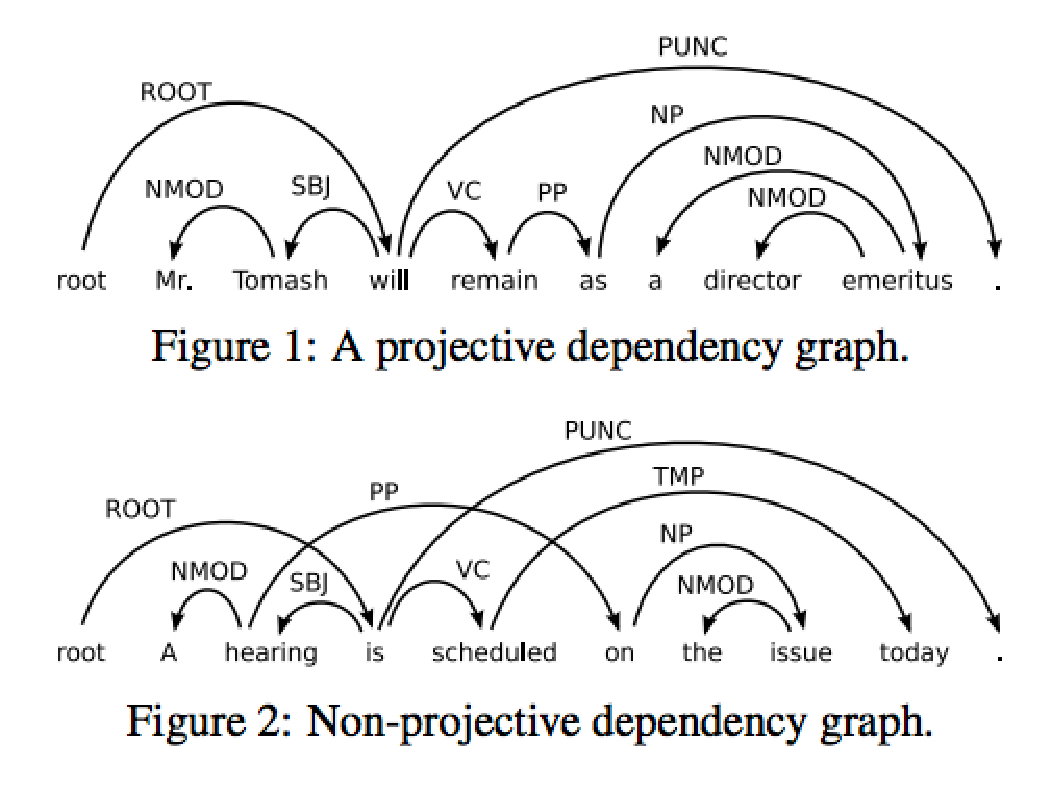
\includegraphics[width=0.85\textwidth]{figures/projectivity.eps}\\
      \footnotesize{(Figure from
        \href{https://languagelog.ldc.upenn.edu/nll/?p=7851}{Language Log:
          Non-projective flavor}.)}
  \end{center}
\end{slide}

\begin{slide}[toc=Dep. advantages]{The advantages of dependency grammars}
  Dependency grammars are becoming the dominant syntactic theory used in NLP,
  since
  \begin{itemize}
  \item dependency trees are in many respect simpler structures than phrase
    structure parse trees (e.g., have only one node per word);
  \item the predicate-argument analysis of sentences provided by dependency
    graphs is a very good starting point for event or frame-oriented semantic
    analysis.
  \end{itemize}
\end{slide}

\begin{slide}[toc=Semantic representation]{Usability for semantic
    representation}
  Compare, for event-semantic aspects
  \begin{small}
  \begin{center}
    \begin{dependency}[theme=simple, edge style={white}, label style={text=white}]
      \begin{deptext}[column sep=1em, nodes={text=white}]
        the \& students \& love \& their \& professors \\
      \end{deptext}
      \depedge{2}{1}{det}
      \depedge{3}{2}{nsubj}
      \depedge{3}{5}{dobj}
      \depedge{5}{4}{poss}
    \end{dependency}
    \Tree[.S [.NP [.Det \textit{the} ]
               [.Noun {\textit{students}} ]]
               [.VP [.Vt {\textit{love}} ]
               [.NP [.Det \textit{their} ]
               [.Noun {\textit{professors}} ]
             ]]]
           \end{center}
         \end{small}
\end{slide}

\begin{slide}[toc=The parsing task]{The dependency parsing task}
  Given a syntactic theory, the parsing task is to assign syntactic structure to
  input sentences which satisfy the constraints/conditions of the theory. For
  dependency grammars, this means assigning a \emph{dependency structure}:
  \begin{itemize}
  \item identifying direct dependencies between words of the sentence,
  \item in such a way that together they constitute a \emph{dependecy tree}
    which satisfies all of the the theory's constraints.
  \end{itemize}
\end{slide}

\begin{slide}[toc=]{The dependency parsing task cont.}
  In modern NLP practice, the dependency grammar underlying a parsing task is
  typically specified implicitly, using a so called \emph{\gold treebank}, that
  is, a dataset consisting of sentences annotated with their parse
  trees.\bigskip

  This makes parsing a \emph{\gold structured supervised learning task}: given a
  training set consisting of a large number of
  $\langle \mathrm{sentence}, \mathrm{parse}~\mathrm{tree} \rangle$ pairs, learn
  to predict the parse tree of unseen sentences.
\end{slide}

\begin{slide}{Performance metrics}
  For dependency grammar parsers, the most commonly used evaluation metrics are
  \begin{itemize}
  \item \emph{\gold UAS (Unlabeled Attachment Score):} The percentage of words that are
    attached to the correct head.
  \item \emph{\gold LAS (Labeled Attachment Score):} The percentage of words that are
    attached to the correct head with the correct dependency label.
  \end{itemize}
\end{slide}

\begin{slide}{Parsing algorithms}
  Like most sequence tagging approaches, dependency parsing algorithms use the
  strategy of breaking down the prediction task into individual decisions over
  elements of the structure. In this case,

  \begin{itemize}
  \item the individual decisions are about individual dependencies between words, and
  \item the central problem is to ensure that the individual decisions lead to a
    coherent dependency tree.
  \end{itemize}
  Dependency parsers typically use either a 
  \begin{itemize}
  \item \emph{\gold transition-based}, or
  \item \emph{\gold graph-based} approach.
  \end{itemize}
\end{slide}

\section{Transition-based parsing}

\begin{slide}[toc=The model]{The transition-based approach}
  The algorithm is based on a formal model of a parsing process which moves from
  left to right in the sentence to be parsed and at every step chooses one of
  the following actions:
  \begin{itemize}
  \item ``assign the current word as the head of some previously seen word,
  \item assign some previously seen word as the head of the current word,
  \item or postpone doing anything with the current word, adding it to a store
    for later processing.''\footnote{\citet[ch. 15]{jurafsky2019speech}.}
  \end{itemize}
\end{slide}

\begin{slide}[toc=]{The transition-based approach}
  The formal model of this process consists of the following component:
  \begin{itemize}
  \item a \emph{\gold buffer}, in which the unprocessed tokens of the input are contained;
  \item a \emph{\gold stack} containing tokens for current operation and storing postponed
    elements;
  \item a \emph{\gold dependency graph}, which is being built for the input
    sentence.
  \end{itemize}
\end{slide}

\begin{slide}[toc=Configurations]{Model configuration}
  The model is in a certain \emph{\gold configuration} at every step of the
  process:
  \begin{center}
    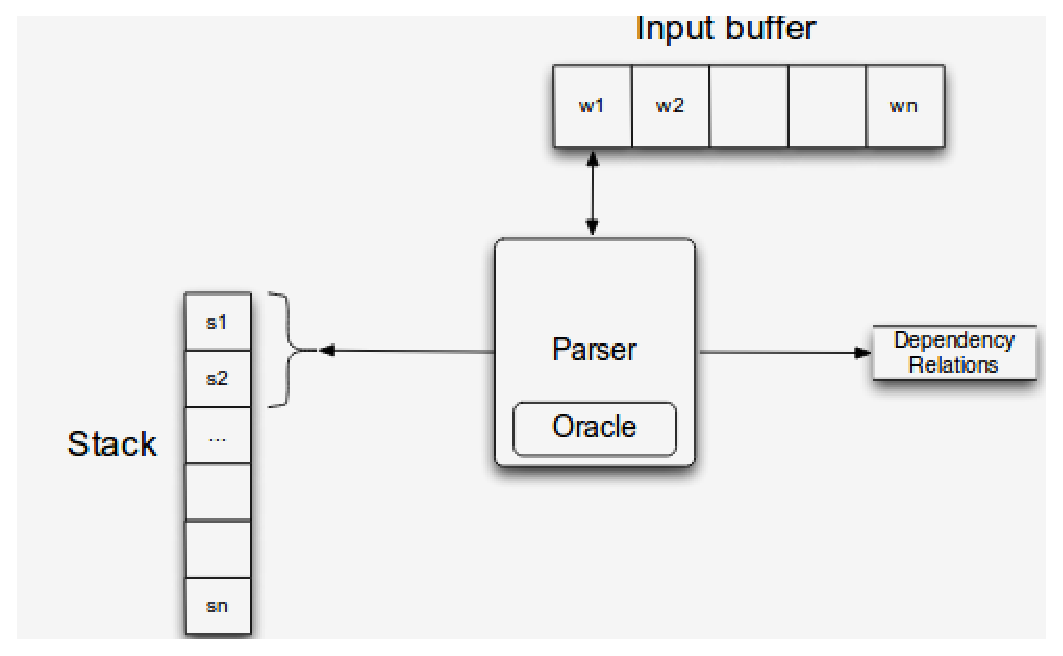
\includegraphics[width=0.85\textwidth]{figures/transition_config.eps}\\
    \footnotesize{(Figure from \citet[ch. 15]{jurafsky2019speech}.)}
  \end{center}
\end{slide}

\begin{slide}[toc=Initial config]{Initial configuration}
  The parsing process starts with the special initial configuration in which
  \begin{itemize}
  \item the buffer contains all words of the input,
  \item the stack contains the single root node of the dependency graph,
  \item and the dependency graph is empty (contains no dependency edges).
  \end{itemize}
\end{slide}

\begin{slide}[toc=Parsing process]{Parsing process}
  At every step, one of the permitted configuration manipulating actions
  (configuration transitions) are performed. The permitted actions vary; a very
  simple set of actions is used in the so called \emph{\gold arc standard}
  approach:
  \begin{itemize}
  \item \emph{\gold left arc with label $l$}: add edge $s_2\xleftarrow{l} s_1$
    to the graph and remove $s_2$ ($s_2$ cannot be the root element);
  \item \emph{\gold right arc with label $l$}: add edge $s_2\xrightarrow{l} s_1$
    to the graph and remove $s_1$ ($s_1$ cannot be the root element);
  \item \emph{\gold shift}: remove the first word $w_1$ from the buffer and put
    it on the top of the stack.
  \end{itemize}
  The process ends when a configuration is reached in which none of the actions
  can be performed.
\end{slide}

\begin{slide}[toc=]{Parsing process cont.}
  The process is guaranteed to end after a finite number of steps, in a
  configuration in which the buffer is empty and the created dependency graph is
  a well-formed dependency tree for the whole input:
  \begin{itemize}
  \item it ends because at every step we decrease the ``collective token
    distance from the dep. graph''
    $2 \cdot \#(\mathrm{tokens~in~buffer}) + \#(\mathrm{tokens~in~stack})$;
  \item the buffer must be empty because otherwise the shift action would be
    available, and the stack can contain only the root element for similar
    reasons;
  \item each input token has exactly one head in the graph;
  \item there cannot be a \emph{circle} in the graph.
  \end{itemize}
\end{slide}

\begin{slide}[toc=]{Parsing process cont.}
  An example run from \citet[ch. 16]{jurafsky2019speech}:
  \begin{center}
        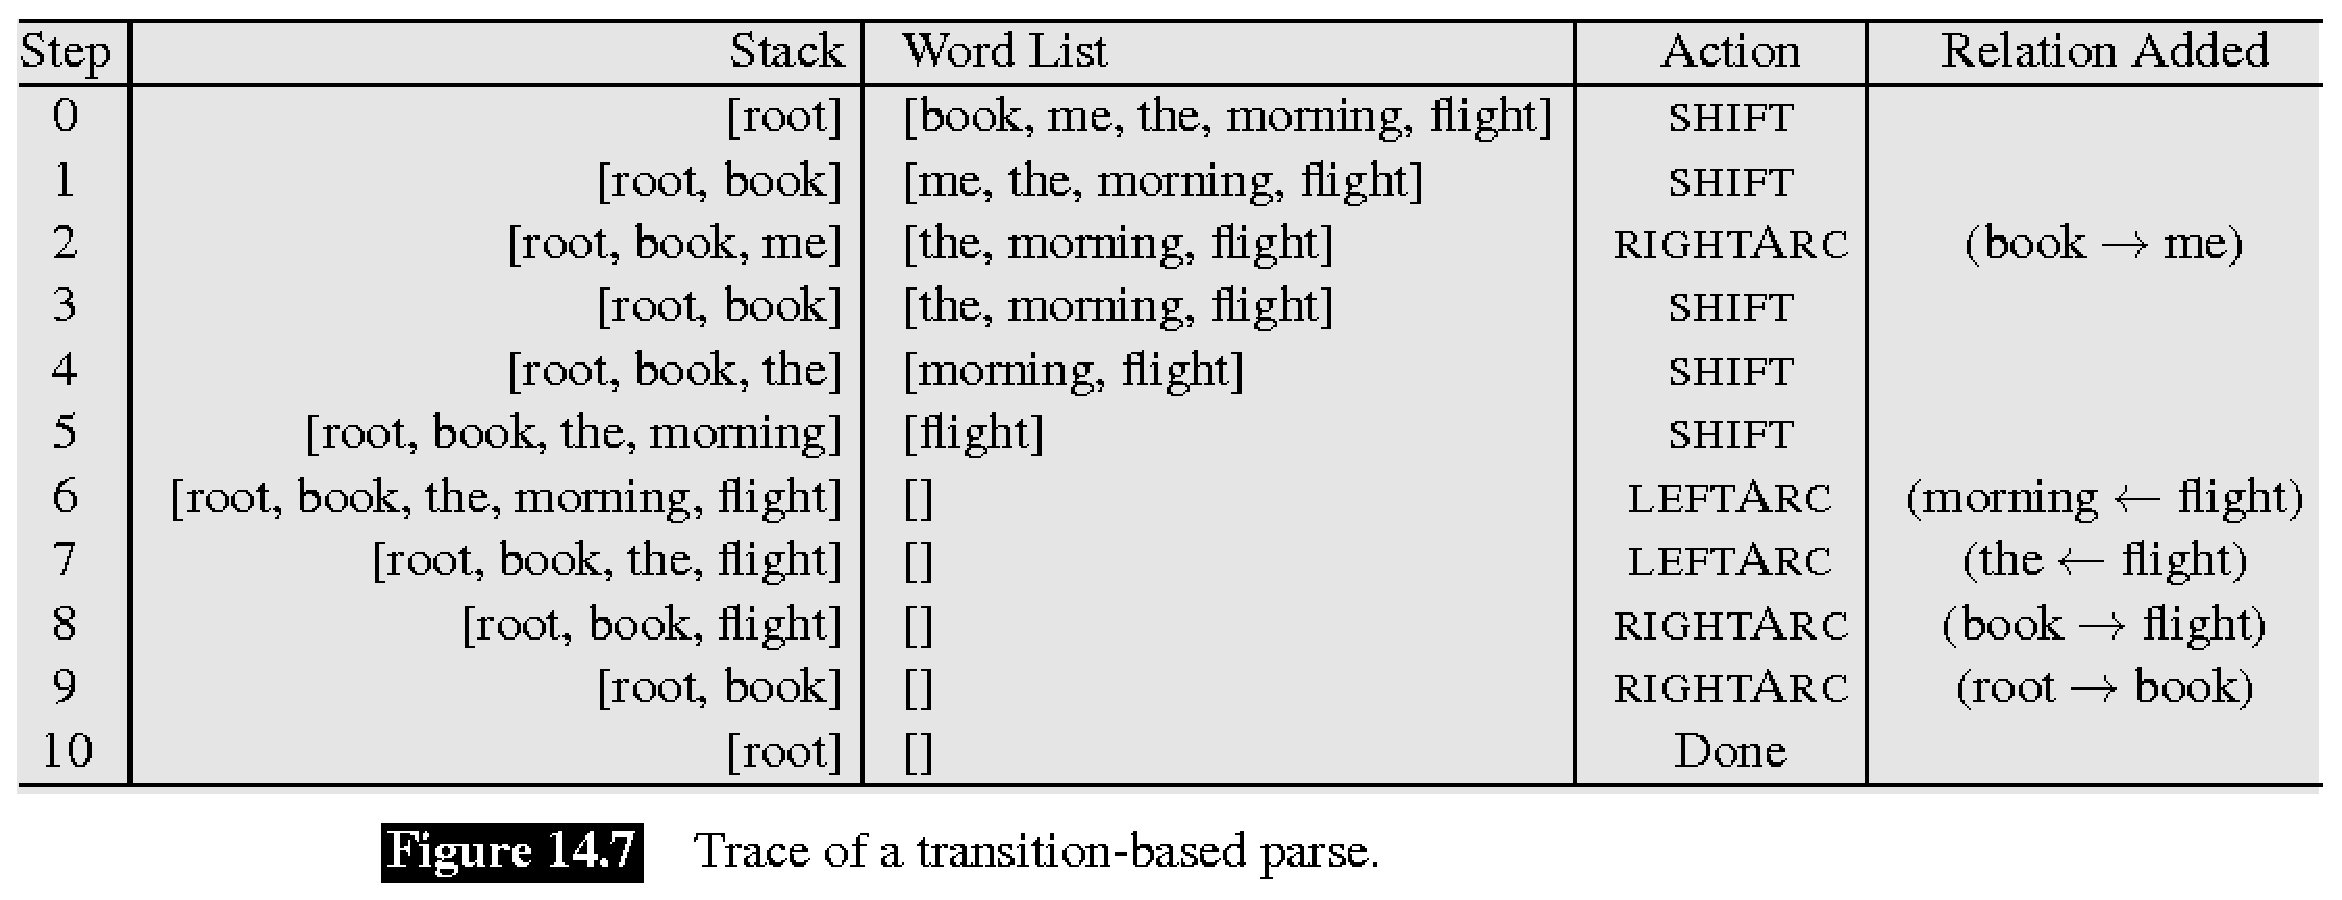
\includegraphics[width=1.\textwidth]{figures/transition_run.eps}\\
  \end{center}
\end{slide}

\begin{slide}[toc=Decision]{Choosing the right action}
  How does a parser decide which action to choose? The model has to act as a
  \emph{\gold classifier over possible configurations}: if there are $n$ labels,
  then there will be $2n+1$ actions/classes.\bigskip
  
  To have training data for this classifier, dependency treebank annotations
  have to be turned into supervised datasets containing
  $$\langle \mathrm{parser~~configuration}, \mathrm{correct~~action} \rangle$$
  pairs, i.e., treebanks have to be turned into datasets about the actions of a
  ``\emph{\gold parsing oracle}'', which always chooses the right action.
\end{slide}

\begin{slide}[toc=Oracle actions]{Converting a parse tree ``to oracle actions''}
  Given the correct parse tree, the configurations and actions of the
  \emph{oracle} can be reconstructed using a straightforward algorithm:
  \begin{itemize}
  \item (obviously) start with the stack containing only the root and a buffer
    with the full input;
  \item choose the \emph{left arc} action with the correct label if it leads to a
    correct edge,
  \item else choose the \emph{right arc} action with the correct label if (i) it
    leads to a correct edge (ii) all dependencies with $s_1$ as head were already
    added to to the dependency graph;
  \item otherwise choose shift.
  \end{itemize}
\end{slide}

\begin{slide}[toc=Other actions]{Alternative action/transitions sets}
  \emph{Arc-standard} is not the only transition system used for
  transition-based parsers -- an important alternative is \emph{\gold
    arc-eager}, which can radically simplify some derivations. Arc-eager has the
  following actions:
  \begin{itemize}
  \item \emph{\gold Right-arc}: add edge $s_1\xrightarrow{l} w_1$ and move $w_1$
    to the top of the stack.
  \item \emph{\gold Left-arc}: add edge $s_1\xleftarrow{l} w_1$ and remove $w_1$
    from the buffer. Precondition: $s_1$ does not have a head yet.
  \item \emph{\gold Shift}: move $w_1$ to the top of the stack.
  \item \emph{\gold Reduce}: remove $s_1$ from the stack. Precondition: $s_1$
    already has a head.
  \end{itemize}
\end{slide}

\begin{slide}[toc=Non-projectivity]{The problem of non-projectivity}
  Arc-standard and arc-eager transitions can produce only projective trees, but
  most treebanks contain a sizeable amount of non-projective sentences:
  \begin{center}
    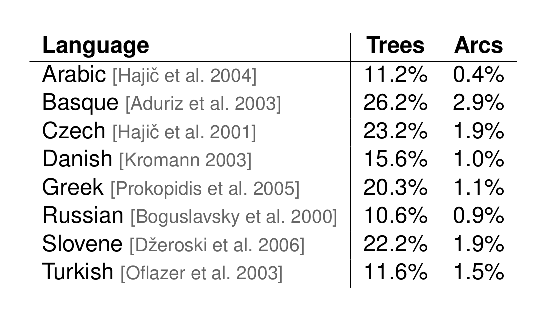
\includegraphics[width=0.85\textwidth]{figures/non-projectivity.eps}\\
    \footnotesize{(Table from \cite{nivre2013beyond}.)}
  \end{center}
\end{slide}

\begin{slide}[toc=]{Non-projectivity: solutions}
  \begin{itemize}
  \item Use transition systems that can create (a certain amount of)
    non-projective edges.
  \item \emph{\gold Pseudo-projective parsing}:
    \begin{itemize}
    \item find a $\varphi$ mapping between all relevant (projective +
      non-projective) trees and projective ones;
    \item for training, the training set is ``projectivized'' using $\varphi$,
      and the parser is trained on the transformed dataset;
    \item for prediction/inference, $\varphi^{-1}$ is applied to the parser's
      output to get the final (possibly non-projective) result.\footnote{See,
        e.g., \cite{nivre-nilsson-2005-pseudo} for details.}
    \end{itemize}
  \end{itemize}
\end{slide}

\begin{slide}[toc=Features]{Classifier features}
  Proper feature extraction from configurations is important for performance.
  Traditional (e.g., perceptron-based) solutions used complex, expert-engineered
  feature templates, e.g.,
  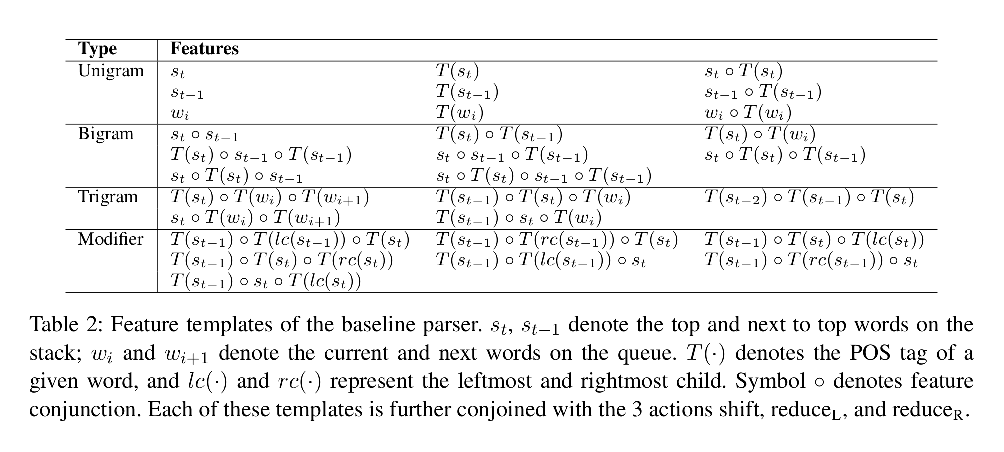
\includegraphics[width=1.\textwidth]{figures/trans_dep_features.eps}\\
  \footnotesize{\hspace{3.4cm}(Table from \cite{huang2009bilingually}.)}
\end{slide}

\begin{slide}[toc=]{Classifier features cont.}
  As in other areas, the problems with manual feature engineering and data
  sparsity led to the development of deep learning solutions, which rely on
  \emph{embeddings} for classification. The Stanford neural dependency parser is
  a simple but representative example:
  \begin{center}
    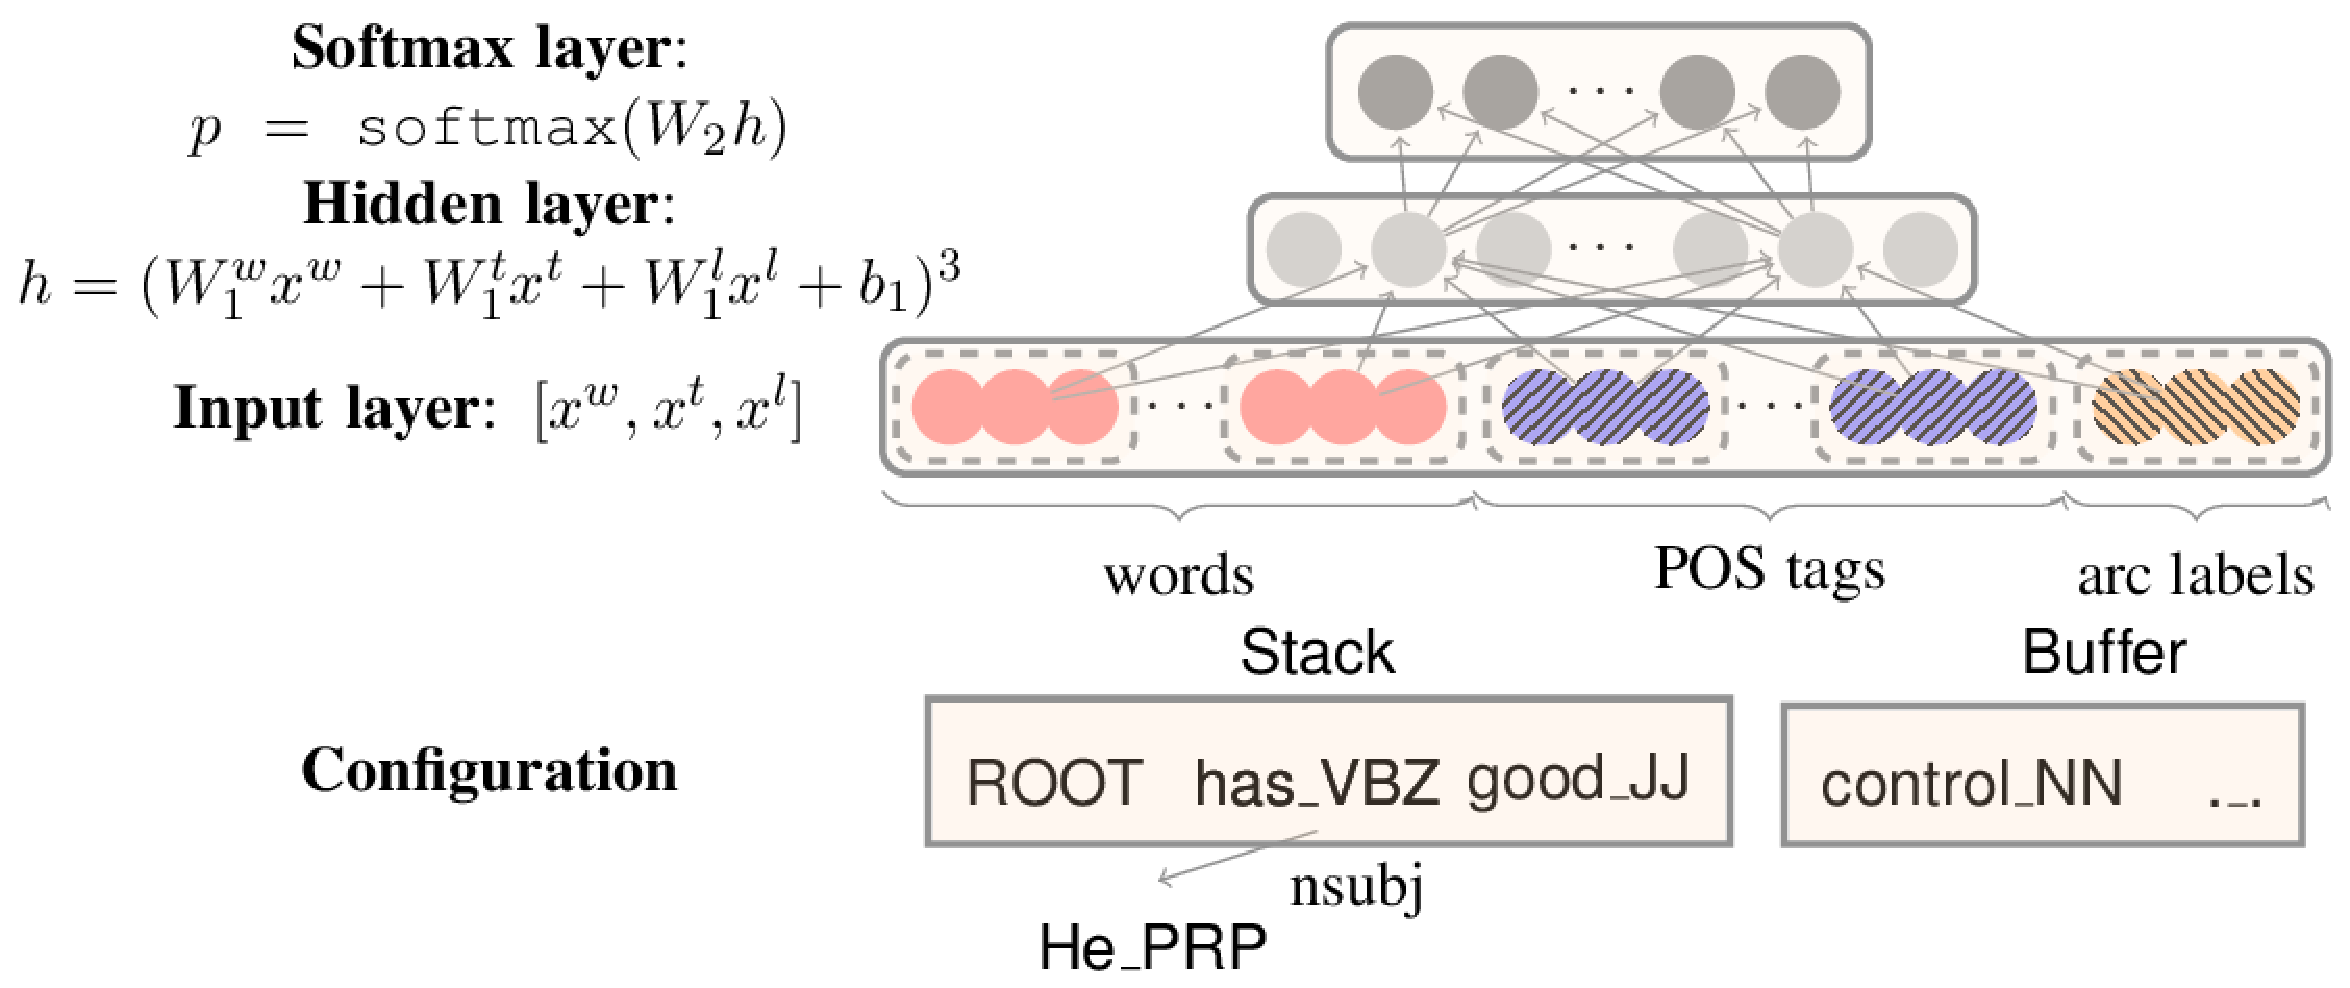
\includegraphics[width=0.8\textwidth]{figures/trans_dep_neural.eps}
    
    \footnotesize{(Figure from  from \cite{chen2014fast}.)}
  \end{center}
\end{slide}

\begin{slide}[toc=]{Architectures}
  The used model architectures are the typical classification architectures used
  in NLP:
  \begin{itemize}
  \item Before the emergence of DL-based parsers, mainly linear models were used
    (with weighted perceptron or SVM as the learning algorithm), but k-NN-based
    solutions also existed.
  \item In deep learning, CNN and LSTM-based models were dominant before the
    appearance of transformer-based solutions, which rely heavily on pretrained
    contextual embeddings such as BERT.
  \end{itemize}
\end{slide}

\section{Graph-based parsing}

\begin{slide}[toc=Approach]{The graph-based approach}
  Two contrasting ways of scoring parse trees:
  \begin{itemize}
  \item The \emph{\gold transition-based} approach transforms the problem of
    scoring a dependency-graph into scoring the \emph{steps} of a somewhat
    complicated \emph{graph building process}.
  \item \emph{\gold Graph-based} parsers, in contrast, score directly the graphs
    themselves and try to find the dependency graph with the maximal score:
  $$\hat g =\underset{g\in G}{\operatorname{argmax}}~S(g)$$
  \end{itemize}
\end{slide}

\begin{slide}[toc=]{The graph-based approach cont.}
A simple but surprisingly well performing approach is to
\begin{itemize}
\item score all the possible edges individually (this requires scoring $n(n-1)l$
  directed edges if there are $n$ tokens and $l$ labels), and then
\item find the (correctly directed) tree with the largest sum total score.
\end{itemize}
The assumption is simply that
$$
S(g) = \sum_{e\in g} S(e).
$$
This way of scoring a graph is called the \emph{\gold edge-} or \emph{\gold
  arc-factored} approach.
\end{slide}

\begin{slide}[toc=Finding the maximum spanning tree]{Finding the tree with the
    maximal score}
  A brute-force search over all possible graphs would be obviously unfeasible.
  Fortunately, there are relatively fast algorithms for finding the maximally
  scoring tree (the so-called \emph{maximum spanning tree}). \bigskip

  A frequently used algorithm is the \emph{\gold Chu--Liu--Edmonds algorithm},
  which has time complexity $\mathcal O( n^3 l)$ for $n$ input tokens and $l$
  possible labels, what can be reduced to $\mathcal O(n^2l)$ by storing the edge
  scores in a special data structure, a so-called Fibonacci-heap.
\end{slide}

\begin{slide}[toc=Edge features]{Edge scoring features}
  Graph-based dependency parsers are \emph{regressors}: they have to produce
  scores for the possible edges between the input tokens. The used feature
  templates are analogous to those in transition-based parsers:
  \begin{itemize}
  \item the dependent and its affixes, POS etc.;
  \item the head and its affixes, POS etc;
  \item the edge label;
  \item the relationship between the head and the dependent in the sentence,
    e.g. their distance;
  \item for neural architectures, embeddings for the nodes and the label of the
    edge.
  \end{itemize}
\end{slide}

\begin{slide}{Architectures}
  Analogously to the transition-based case, both classic ML and neural
  graph-based parsers have been developed over the years, the highest performing
  parsers using self-attention layers.\bigskip

  An important aspect of some of the recent architectures, introduced by a paper
  by \cite{dozat2016deep}, is that they use different sets of embeddings for the
  head and dependent representations of the same words.
\end{slide}


\begin{slide}[toc=Trade-offs]{Transition- vs graph-based parsing}
There are important trade-offs between the two approaches.\bigskip

\emph{\gold Time complexity}: the time-complexity of parsing $n$ tokens with $l$
possible edge labels is

\begin{itemize}
\item typically $\mathcal O (n)$ for transition-based parsers, while
\item graph-based parsers precompute scores for all possible edges, so they
  start with an $\mathcal O(n^2 l)$ operation, and the time of finding the
  maximum spanning tree is added to this. Even if we treat finding labels as a
  separate task the $\mathcal O(n^2)$ complexity is inescapable.
\end{itemize}
\end{slide}

\begin{slide}[toc=]{Transition- vs graph-based parsing cont.}
\emph{\gold Non-projectivity}: as we have seen, non-projectivity is a serious problem
for the most wide-spread transition systems which needs special treatment.
Graph-based approaches don not suffer from this problem.\bigskip

\emph{\gold Performance}: Transition-based systems tend to have problems with
long-distance dependencies, graph-based models do not have this performance
issue. As a consequence, the dependency parser leader boards are dominated by
graph-based systems.
\end{slide}
\section{References}

\begin{slide}{References}
  \bibliographystyle{plainnat}
  \nobibliography{nlp_course.bib}
  \begin{footnotesize}

    \bibentry{chen2014fast}.\medskip

    \bibentry{dozat2016deep}.\medskip

    \bibentry{huang2009bilingually}.\medskip
    
    \bibentry{jurafsky2019speech}.\medskip

    \bibentry{koopman2013introduction}.\medskip
    
  \end{footnotesize}
\end{slide}

\begin{slide}[toc=]{References cont.}
  \begin{footnotesize}

    \bibentry{nivre-nilsson-2005-pseudo}.\medskip

    \bibentry{nivre2013beyond}.\medskip
    
  \end{footnotesize}
\end{slide}

\end{document}

%%% Local Variables:
%%% mode: latex 
%%% TeX-master: t
%%% End:

% LocalWords:  Tokenization Discriminative discriminative
